\section{Results}

\subsection{Microsimulation Non-take-up}
Our microsimulation results indicate that the non-take-up-rate of BAföG, among theoretically eligible students ranged from approximately 50--70\% across the survey years 2007--2021, with an average of 60\%  (Table \ref{table:microsimulation-ntu}).

These estimates are broadly in line with previous findings on non-take-up of social benefits in Germany, which generally falls between 40--67\%, depending on the program and time period (see Table \ref{table:NTU-studies}). 
While our estimates are broadly consistent with prior research, they are noticeably higher than the 36--40\% non-take-up rate for BAföG reported by \cite{herber_non-take-up_2019}, who also use SOEP survey data, but for the period 2002--2013.

This discrepancy may be attributable to several factors, including differences in the estimation of theoretical eligibility. These factors include the specific SOEP variables used to capture income and reported BAföG receipt, the time periods under study (with our analysis covering 2007--2021, compared to \cite{herber_non-take-up_2019}, which covers 2002--2013), as well as other differences in the microsimulation design and modeling approach.



\begin{table}[htbp]
\footnotesize
\centering
\begin{tabular}{l@{\hspace{2em}}r@{\hspace{2em}}r}
\toprule
\textbf{Year} & \textbf{Non-Take-Up}  &  \textbf{Beta Error}  \\
              & \(\Pr(\text{NTU} =1\,|\,\text{M} = 1)\) & \(\Pr(\text{TU} = 1\,|\,\text{M} = 0)\) \\
\midrule
2007 & 60.6 & 13.6 \\
2008 & 63.5 & 17.1 \\
2009 & 61.0 & 18.6 \\
2010 & 60.9 & 17.7 \\
2011 & 53.8 & 16.1 \\
2012 & 51.5 & 18.9 \\
2013 & 50.0 & 15.9 \\
2014 & 55.1 & 16.1 \\
2015 & 64.0 & 12.6 \\
2016 & 56.5 & 12.4 \\
2017 & 62.6 & 10.1 \\
2018 & 63.9 & 15.3 \\
2019 & 67.5 & 11.7 \\
2020 & 63.7 & 13.6 \\
2021 & 66.7 & 12.3 \\
\midrule
\textbf{Average} & \textbf{59.7} & \textbf{15.3} \\
\bottomrule
\end{tabular}
\caption{Non-Take-Up and Beta Error Rates by Survey Year (\%). Non-take-up is the share of theoretically eligible students (\(M=1\)) who do not receive BAföG; beta error is the share of theoretically ineligible students (\(M=0\)) who do receive BAföG.}
\caption*{\small{Notes: SOEP v39, 2007--2021, weighted with individual weights}}
\label{table:microsimulation-ntu}
\end{table}


\begin{figure}[htbp]
  \centering
  \begin{subfigure}[t]{0.48\linewidth}
    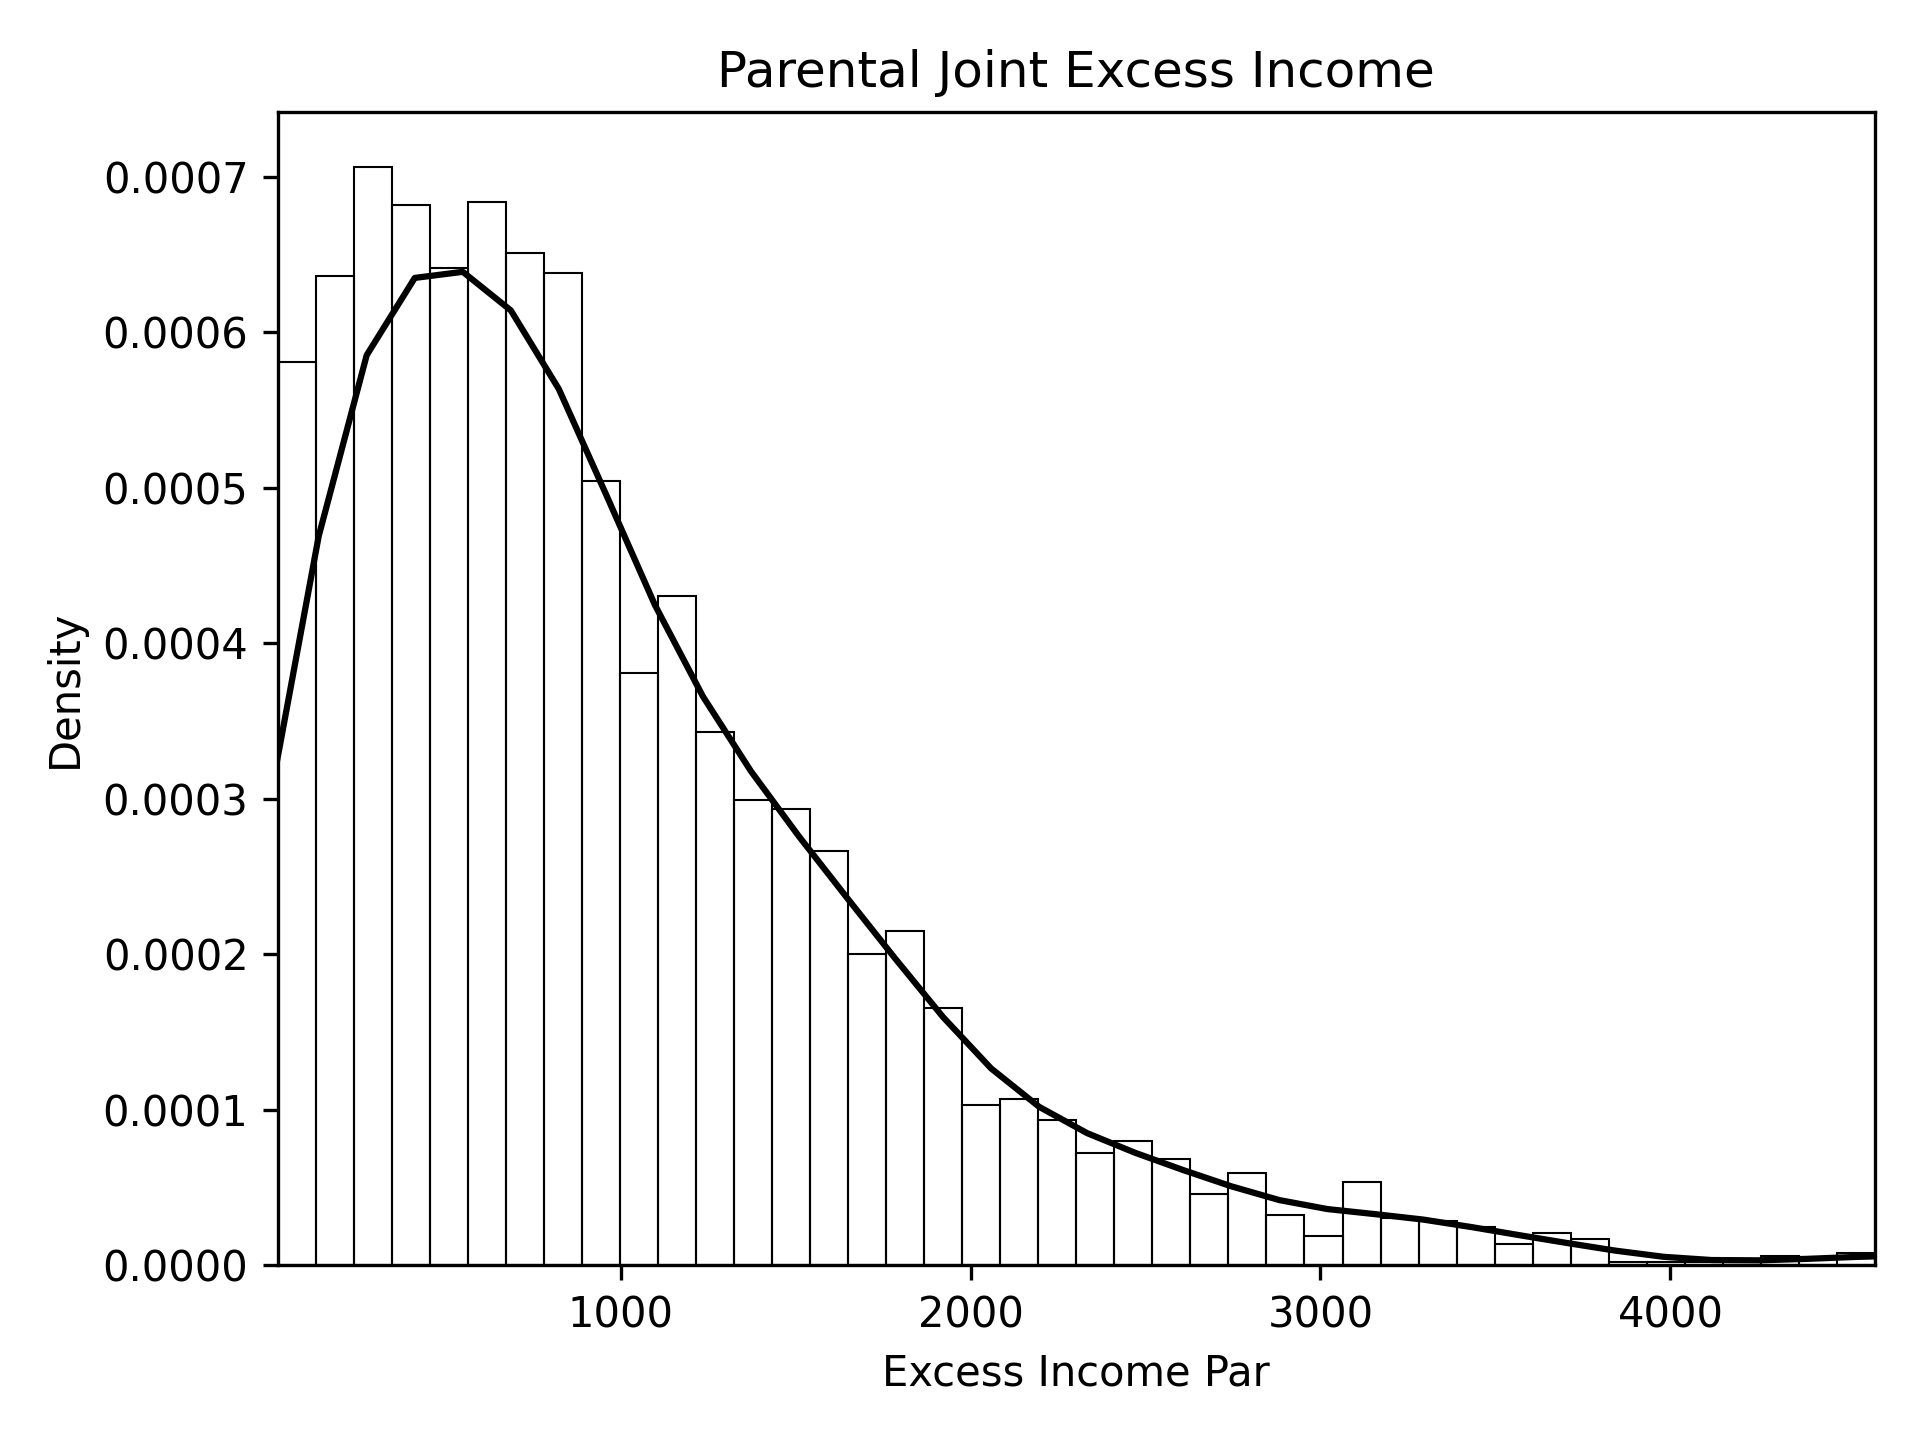
\includegraphics[width=\linewidth]{parental_joint_excess_income_pdf.png}
    \caption{Parental joint excess income}
    \label{fig:parental-excess}
  \end{subfigure}
  \hfill
  \begin{subfigure}[t]{0.48\linewidth}
    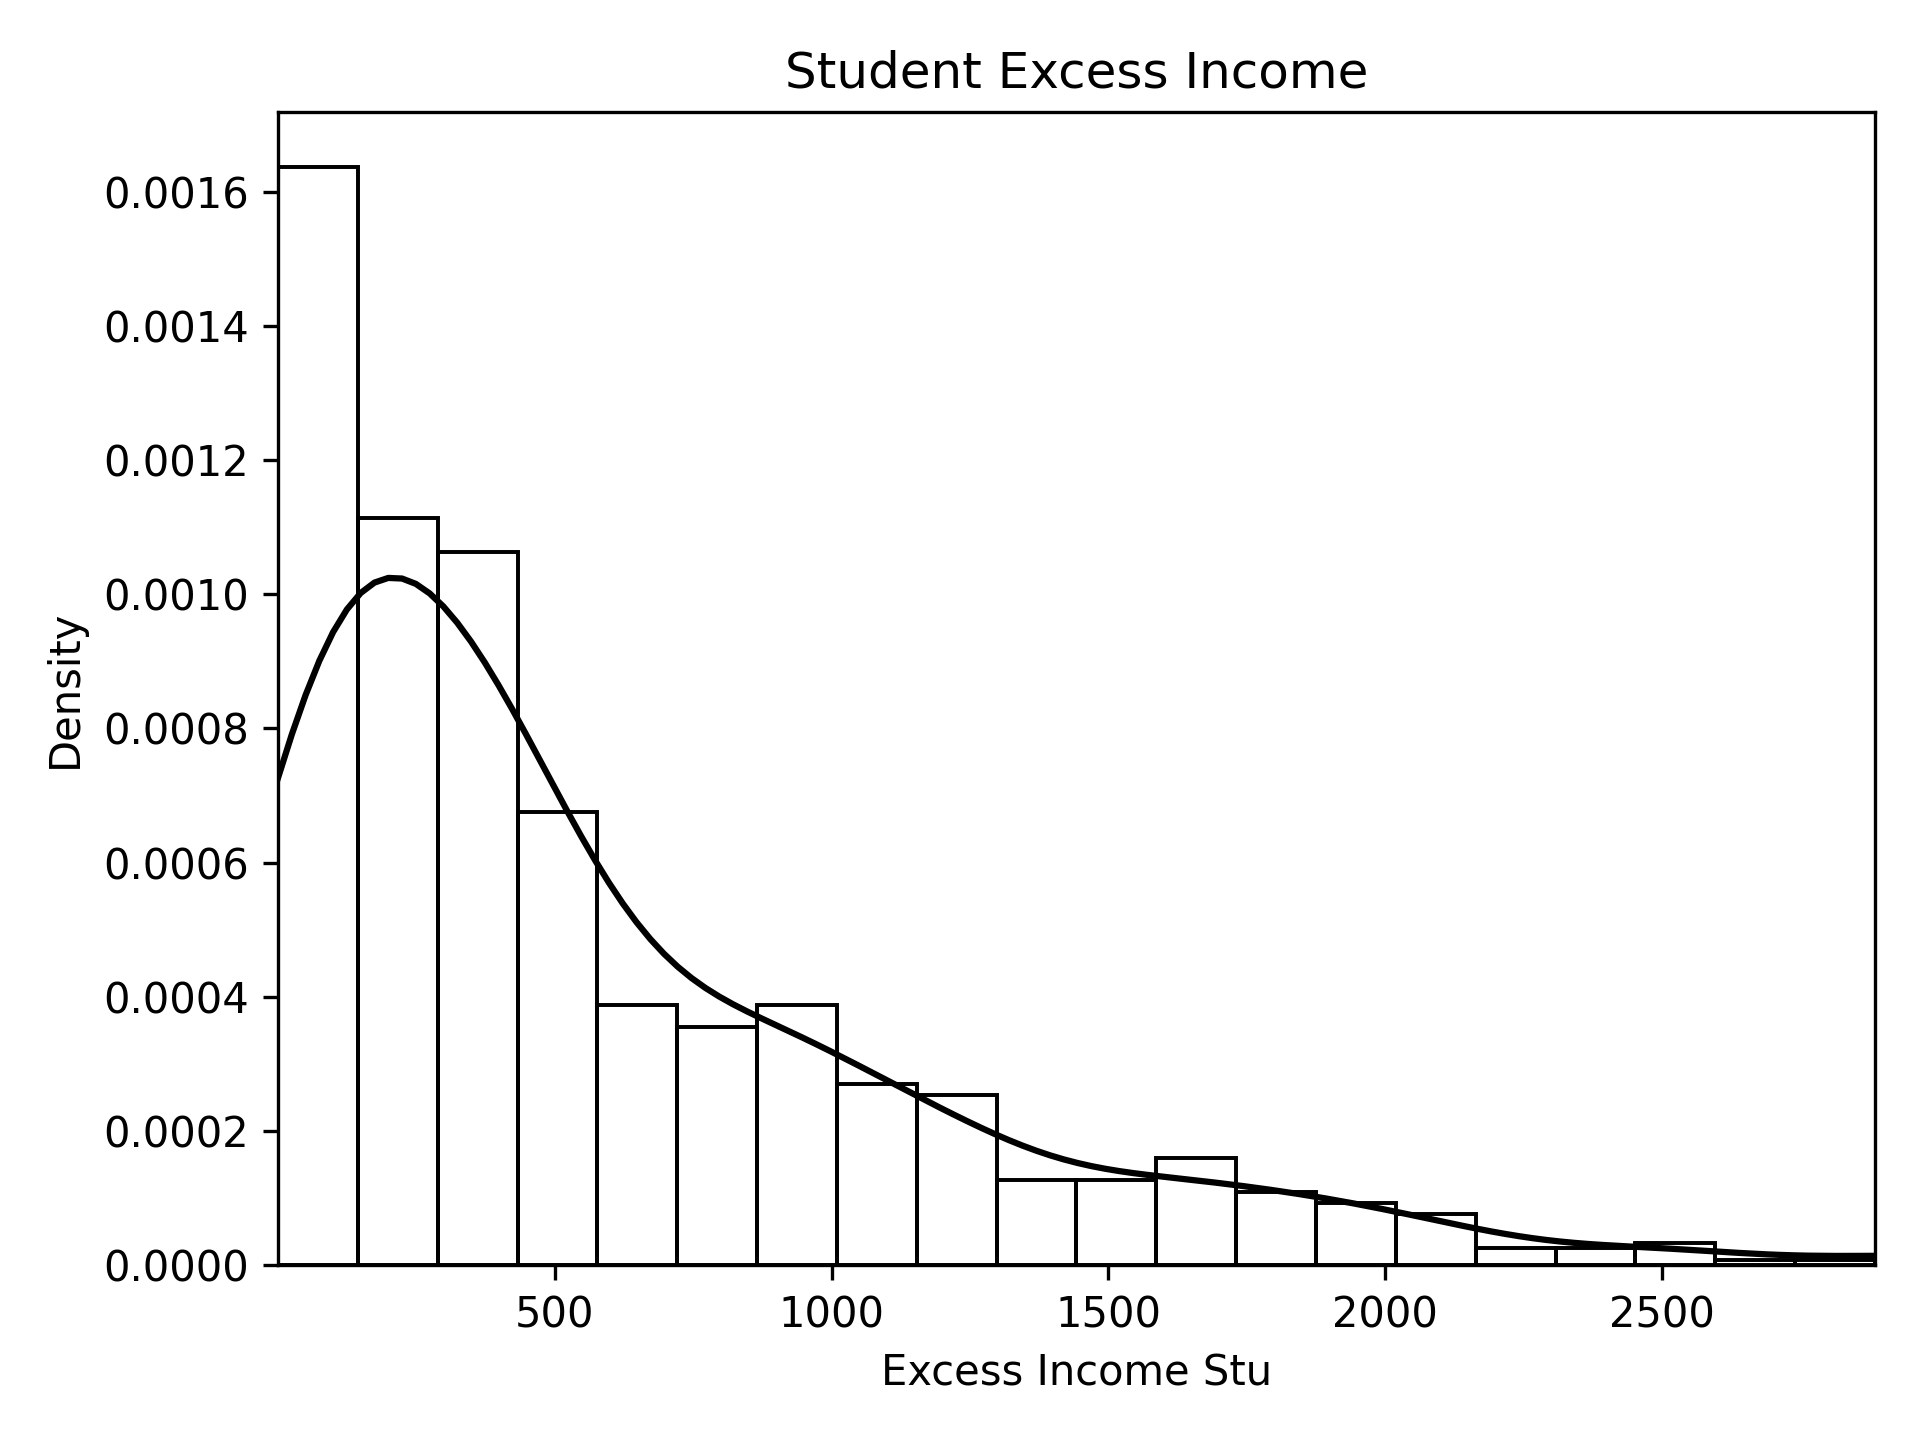
\includegraphics[width=\linewidth]{student_excess_income_pdf.png}
    \caption{Student excess income}
    \label{fig:student-excess}
  \end{subfigure}
  \caption{Simulated mean excess income for parents (\subref{fig:parental-excess}) and students (\subref{fig:student-excess}).}
  \label{fig:excess-income}
\end{figure}

\begin{figure}[htbp]
  \centering
  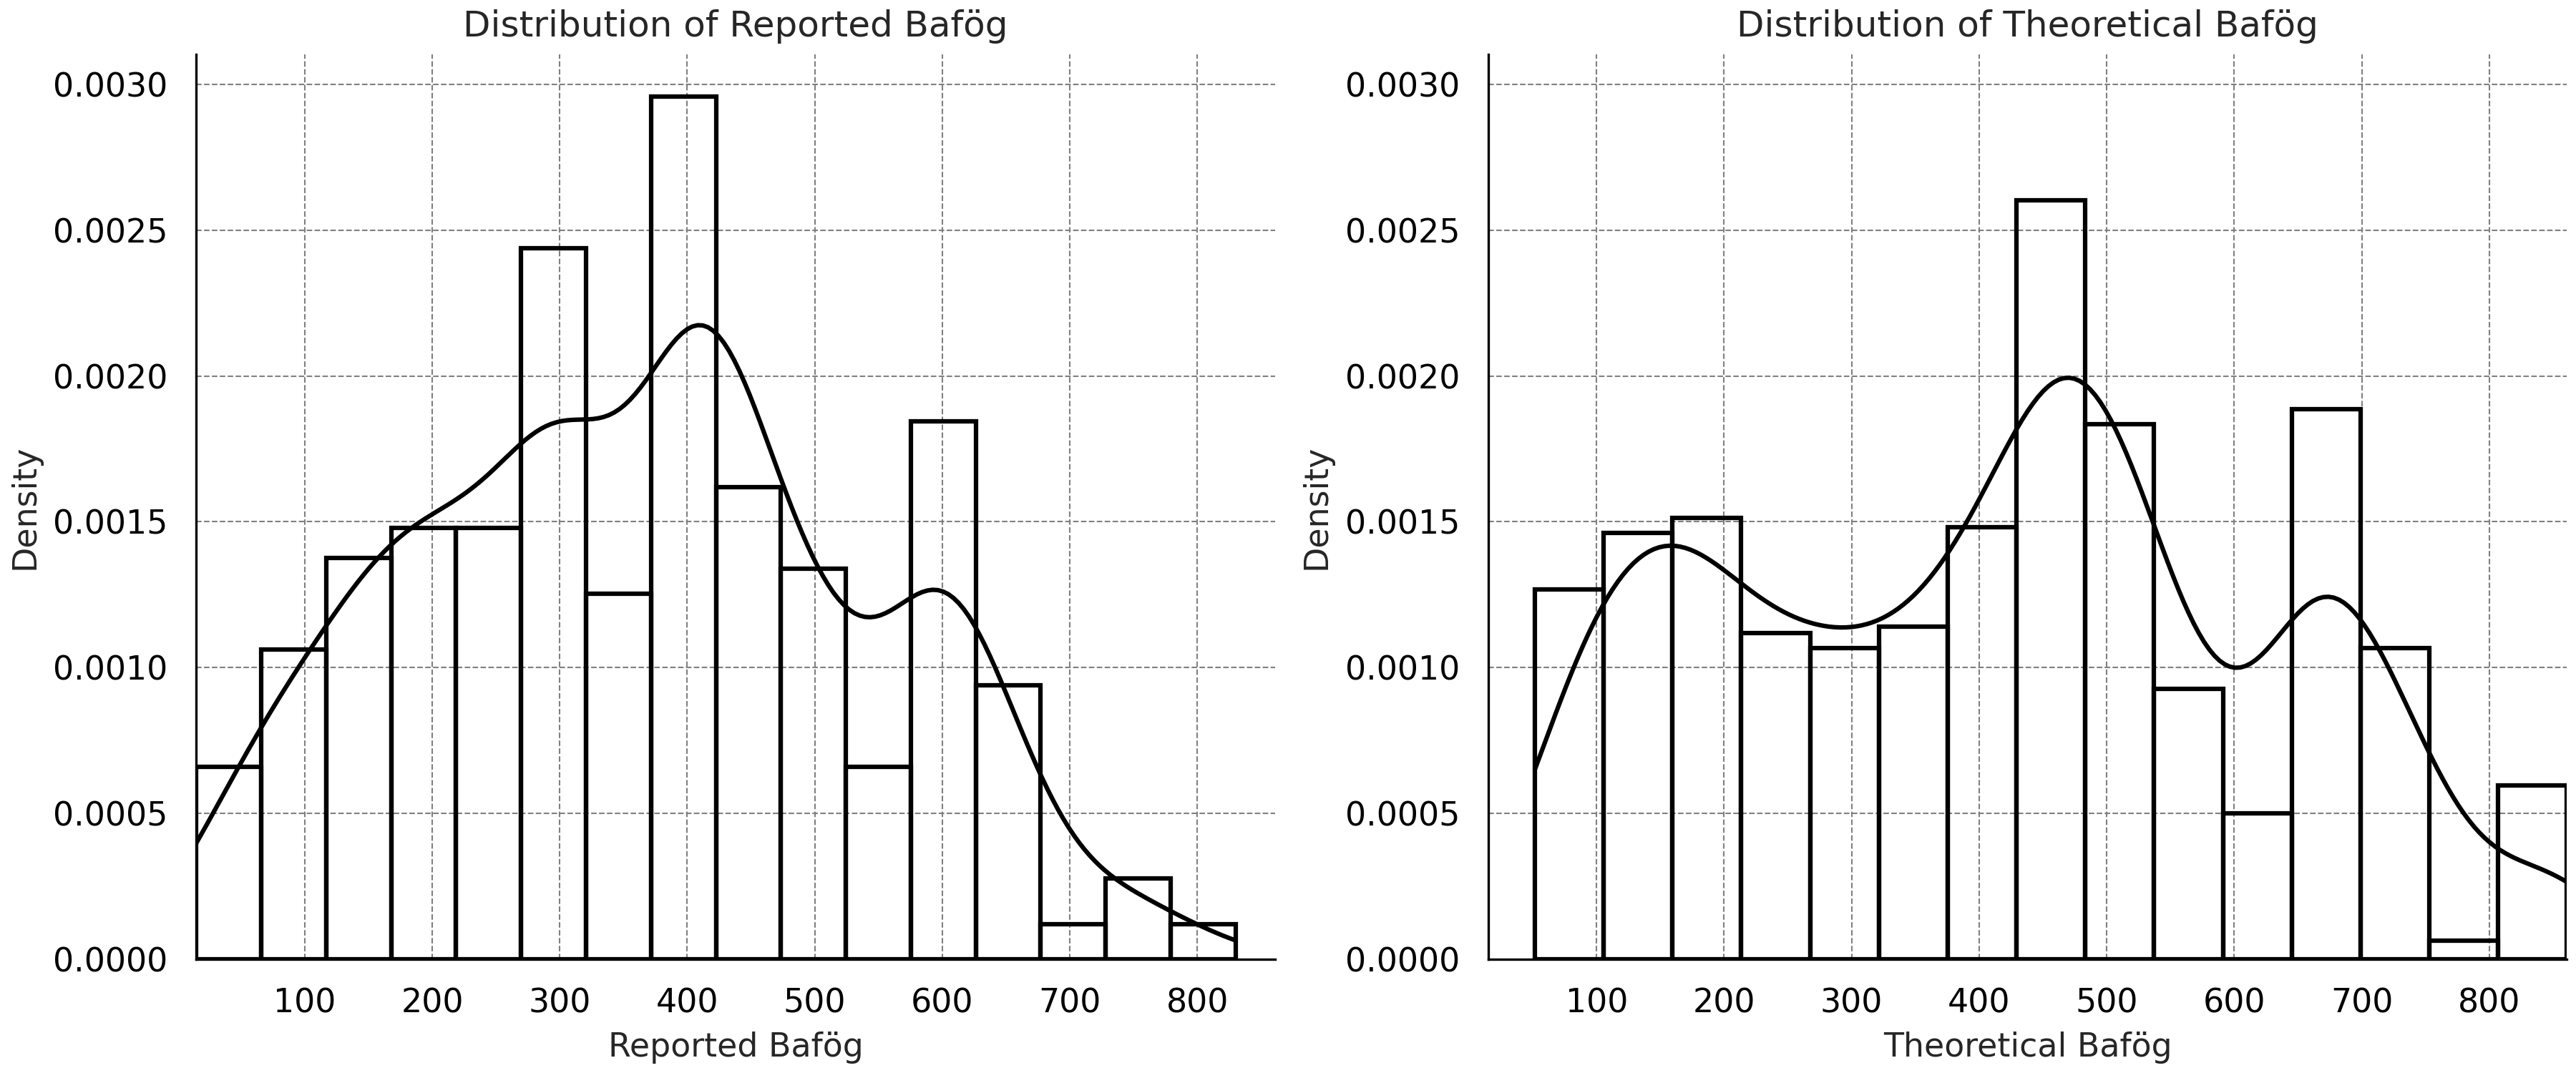
\includegraphics[width=0.95\linewidth]{theo_vs_reported_distribution.png}
  \caption{Comparison of the distribution of reported BAföG receipt in the SOEP-Core sample with the simulated (theoretical) distribution of simulated BAföG entitlements from our model.}
  \label{fig:theo-vs-reported}
\end{figure}

\subsection{Determinants of Non-take-up}
\subsubsection{Binary Choice Model}

\begin{table}
\renewcommand{\arraystretch}{1.25}
\footnotesize
\label{tab:logit-probit-ame}
\begin{tabular}{lllllllll}
\toprule
 & \multicolumn{4}{c}{Logit} & \multicolumn{4}{c}{Probit} \\ 
\cmidrule(lr){2-5} \cmidrule(lr){6-9}
 & Coef. & SE & AME & SE & Coef. & SE & AME & SE \\
 \midrule
Age                           & 0.165**     & 0.081051 & 0.029** & 0.014 & 0.093** & 0.043895 & 0.028** & 0.013 \\
Female                        & 0.526       & 0.353755 & 0.093 & 0.062 & 0.320 & 0.204400 & 0.096 & 0.061 \\
Migration background          & 0.311       & 0.370026 & 0.055 & 0.065 & 0.180 & 0.223065 & 0.054 & 0.066 \\
Has partner                   & 0.815       & 1.092158 & 0.144 & 0.193 & 0.532 & 0.582731 & 0.159 & 0.174 \\
Lives at home                 & 0.421       & 0.389459 & 0.074 & 0.068 & 0.257 & 0.222614 & 0.077 & 0.066 \\
Log Parental Income           & -0.200      & 0.261063 & -0.035 & 0.046 & -0.107 & 0.147114 & -0.032 & 0.044 \\
Log Gross income              & 0.626**     & 0.266827 & 0.110** & 0.046 & 0.372** & 0.148019 & 0.111*** & 0.043 \\
Simulated BAföG amount        & -0.002*     & 0.001047 & -0.000* & 0.000 & -0.001* & 0.000598 & -0.000* & 0.000 \\
Constant                      & -5.578*     & 3.354795 &  &  & -3.307* & 1.926467 &  &  \\
\midrule
\multicolumn{9}{l}{\textbf{Control variables:}} \\
Sibling claimed BAföG before  & -0.398      & 0.324193 & -0.070 & 0.056 & -0.222 & 0.188722 & -0.066 & 0.056 \\
East background               & -1.411***   & 0.434825 & -0.249*** & 0.072 & -0.872*** & 0.260895 & -0.260*** & 0.073 \\
Parents are highly educated   & 0.400       & 0.436344 & 0.070 & 0.077 & 0.252 & 0.249219 & 0.075 & 0.074 \\
\midrule
\multicolumn{9}{l}{\textbf{Time invariant:}} \\
Risk Appetite                 & 0.022       & 0.036996 & 0.004 & 0.006 & 0.012 & 0.023215 & 0.004 & 0.007 \\
\bottomrule
\end{tabular}
\caption{Logit/Probit coefficients and AMEs (Average Marginal Effects). Significance: $^{*} p < 0.1$, $^{**} p < 0.05$, $^{***} p < 0.01$.}
\end{table}


\paragraph{Risk attitudes.} In this analysis, a variable for students' self-assessed willingness to take risks is included. Even though BAföG offers relatively safe and generous conditions, some students might still be hesitant to take on any form of debt if they are generally risk-averse. By including this variable, we aim to capture whether differences in individual risk preferences help explain why some eligible students choose not to apply.

Herber and Kalinowski (2016) also include a risk preference variable in their study, mainly to control for the possibility that risk attitudes could affect take-up behavior or influence how other factors, like impatience, play a role. They do not find a strong effect of risk aversion on BAföG take-up, but they still argue it is useful to control for \citep{herber_non-take-up_2019}. In a similar way, we include this variable to improve our model and to see whether risk aversion plays any role in students’ decisions to reject BAföG.

\paragraph{East German socialization.}  A variable indicating whether the student lives in East Germany is included to account for potential differences in attitudes toward state support rooted in historical and regional context. Alesina and Fuchs-Schündeln (2007) show that individuals from the former GDR tend to have stronger preferences for redistribution and a greater belief in the role of the state in providing social services, and that these differences in preferences can persist for one to two generations after reunification \citep{alesina_good-bye_2007}. Current residence in East Germany may reflect continued exposure to these norms and institutions and can serve as a reasonable proxy for this form of socialization. Since the variable is statistically significant at the 5\% level in our model, we interpret it as capturing persistent regional differences in how students view and respond to publicly provided financial support like BAföG.

\paragraph{Sibling prior experience with BAföG.} An indicator for whether the student has an older sibling who previously received BAföG is included to capture potential differences in access to informal support and familiarity with the application process. Students with siblings who have already gone through the steps of applying may be more aware of eligibility rules and practical requirements. Herber and Kalinowski (2016) highlight that such sibling experience can help reduce informational and procedural barriers, making it more likely that students follow through with the application \citep{herber_non-take-up_2019}. This variable is intended to reflect how previous exposure to the system within the family can shape students’ confidence and ability to navigate what is often perceived as a complex process.

\paragraph{Migration background.} A variable for migration background is included to explore whether differences in familiarity with the BAföG system may influence take-up. Some students may come from households with less exposure to German administrative processes or financial aid structures, which could affect their understanding of eligibility or the application itself. In addition, studies show that individuals with a migration background in Germany often have lower financial literacy, which may make it harder to evaluate financial aid options like BAföG \citep{Tsegay_2024}. Including this variable helps capture potential structural or informational factors that may contribute to lower take-up rates among eligible students. 

\textcolor{red}{FIRST OR SECOND GENERATION MIGRATION BACKGROUND SOEP VARIABLE IS DIRECT OR INDIRECT (MIG BACK 2 IS DIRECT AND 3 IS INDIRECT. THE SOEP VARIABLE NAME IS MIGBACK)}

\textcolor{red}{ALEX: X many background variables on parental education are included. They are derived/ found from… blabla.
Parental education background is shown to have an effect on the student’s decision of take-up, although this is only true for the variable that is conditioned on at least one parent having a masters degree.}

...

\paragraph{Interpretation of Average Marginal Effects from the Probit Model.} All interpretations below are based on the average marginal effects (AMEs) from the Probit model presented in Table 3.

Student age is found to be significantly associated with NTU of BAföG. On average, each additional year of age increases the probability of NTU by 2.8 percentage points, holding all other variables constant. Similarly, student income has a significant effect, as a 100 EUR increase in gross monthly income is associated with a 1.2 percentage point increase in the probability of NTU, suggesting that higher-earning students may be less inclined to rely on BAföG support. Parental income matters as well. A 100 EUR increase in parental gross monthly income is associated with a 0.6 percentage point increase in the probability of NTU. \textcolor{red}{NOTE: LOOK BETTER INTO THIS. AME POSITIVE FOR STUDENTS BUT NEGATIVE FOR PARENTS, DON’T THINK IT IS INTERPRETED CORRECTLY HERE ABOVE, ALSO WHY IS IT DIFFERENT? DOES THAT MAKE SENSE?}

Other variables that have to do with family background were also found to have an effect. For example, having an older sibling who previously received BAföG reduces the probability of NTU by 9.6 percentage points on average, suggesting that familiarity with the system encourages take-up. Migration background is significant only for students with an indirect migration background (those born in Germany to foreign-born parents). For this group, the probability of NTU is 8 percentage points lower on average compared to those without a migration background.  Gender, partnership status, and household size do not appear to significantly affect NTU.

Students from East Germany are much less likely to forgo BAföG than their West German counterparts. The results show that having an East German background decreases the probability of NTU by about 25.9 percentage points, on average. This substantial difference could reflect regional variation in attitudes towards public support or perceived entitlement.

Furthermore, parental education seems to matter, particularly at the highest levels. Having at least one parent with a level 7 ISCED education (equivalent to a master’s degree \textcolor{red}{IS THIS CORRECT?}
) increases the likelihood of NTU by 47.8 percentage points. The effects of lower education levels are not statistically significant in the model.

Lastly, the estimated theoretical BAföG amount is negatively associated with NTU. A 100 EUR increase in the theoretical amount corresponds to a 2.3 percentage point decrease in the probability of NTU, suggesting that higher expected benefits increase take-up. \textcolor{red}{PLEASE CONFIRM THAT THIS MAKES SENSE ALEX}

\begin{figure}[htbp]
  \centering
  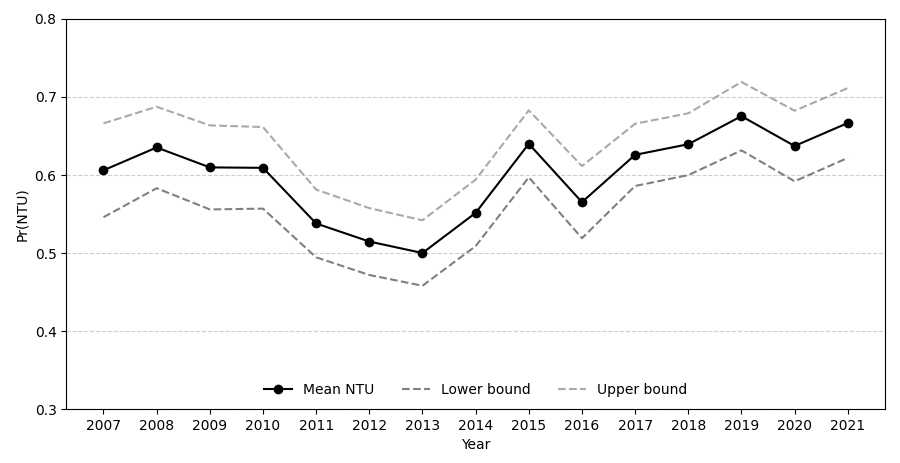
\includegraphics[width=0.75\linewidth]{ntu_bounds.png}
  \caption{Development of the probability of non-take-up from 2007--2021.}
  \label{fig:ntu_bounds_over_years}
\end{figure}

